% ============================================================================
%  Standalone one-slide explainer for the manipulability measure
%      w = sqrt(det(J J^T))   [Yoshikawa 1985]
%  Matches the deck in slides.tex (metropolis, 16:9).
%  Build:  cd docs/latex && pdflatex manipulability_slide.tex
%  To fold into the deck: copy the \begin{frame}...\end{frame} block into slides.tex.
% ============================================================================
\documentclass[aspectratio=169]{beamer}

\usetheme{metropolis}
% \usetheme{Madrid}   % portable fallback if metropolis is not installed

\usepackage{amsmath,amssymb}
\usepackage{tikz}

% Force a pure white background on every slide (metropolis defaults to off-white)
\setbeamercolor{background canvas}{bg=white}

\begin{document}

\begin{frame}{Manipulability: how dexterous is a posture?}
  \begin{equation*}
    w \;=\; \sqrt{\det\!\left(J J^{\top}\right)}
    \qquad\text{[Yoshikawa 1985]}
  \end{equation*}
  \vspace{-0.3em}
  \begin{columns}[T]
    % ---- Left: what the symbols mean ----
    \begin{column}{0.56\textwidth}
      \footnotesize
      \begin{itemize}
        \item $J$ --- the arm's \textbf{Jacobian} at configuration $q$, mapping
              joint rates to tool velocity: $\dot{x} = J\,\dot{q}$
              (here $6\times 8$: 6-DOF pose, 8-DOF chain).
        \item $J J^{\top}$ collapses the rectangular $J$ into a $6\times6$ matrix
              whose determinant we can take.
        \item $w$ is the \textbf{volume of the manipulability ellipsoid} ---
              the tool velocities reachable from a unit sphere of joint rates
              ($w=\sigma_1\sigma_2\cdots\sigma_6$, the singular values of $J$).
      \end{itemize}
      \vspace{0.3em}
      \begin{itemize}
        \item[\textcolor{red!70!black}{$\blacksquare$}] \textbf{Large $w$}: fat, round
              ellipsoid --- moves easily in any direction (dexterous).
        \item[\textcolor{blue!70!black}{$\blacksquare$}] \textbf{Small $w\!\to\!0$}:
              ellipsoid collapses --- near a \textbf{singularity}, IK ill-conditioned.
      \end{itemize}
    \end{column}
    % ---- Right: the ellipsoid intuition ----
    \begin{column}{0.44\textwidth}
      \centering
      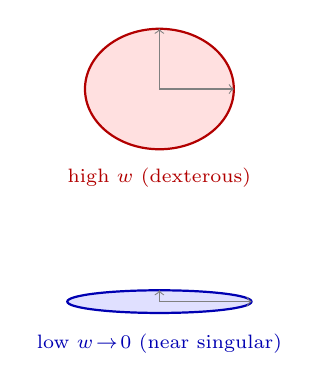
\begin{tikzpicture}[scale=0.9]
        % dexterous (round) ellipse
        \begin{scope}[shift={(0,1.0)}]
          \draw[fill=red!12,draw=red!70!black,thick] (0,0) ellipse (1.05 and 0.85);
          \draw[->,gray] (0,0) -- (1.05,0);
          \draw[->,gray] (0,0) -- (0,0.85);
          \node[red!70!black,font=\scriptsize] at (0,-1.25)
            {high $w$ (dexterous)};
        \end{scope}
        % singular (flat) ellipse
        \begin{scope}[shift={(0,-2.0)}]
          \draw[fill=blue!12,draw=blue!70!black,thick] (0,0) ellipse (1.3 and 0.16);
          \draw[->,gray] (0,0) -- (1.3,0);
          \draw[->,gray] (0,0) -- (0,0.16);
          \node[blue!70!black,font=\scriptsize] at (0,-0.6)
            {low $w\!\to\!0$ (near singular)};
        \end{scope}
      \end{tikzpicture}
      \\[0.3em]
      {\scriptsize Manipulability ellipsoid: axes = singular values of $J$.}
    \end{column}
  \end{columns}
  \vspace{0.4em}
  \hrule height 0.3pt
  \vspace{0.3em}
  {\footnotesize \textbf{In this work:} $w$ is stored per GNG node (map quality
  layer, Fig.~4) and enters the energy cost $J$ with a \emph{minus} sign, so a more
  dexterous candidate scores cheaper.}
\end{frame}

\end{document}
